\documentclass[10pt]{standalone}
\usepackage{commands}
\begin{document}
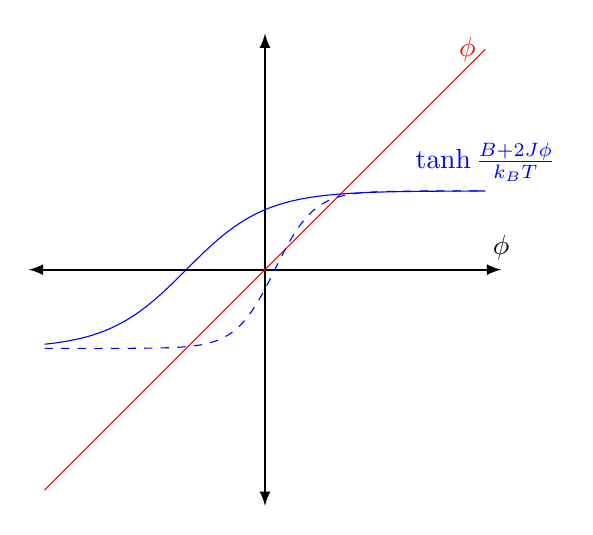
\begin{tikzpicture}
    \draw[latex-latex, thick] (0, -3) -- (0, 3);
    \draw[latex-latex, thick] (-3, 0) -- (3, 0);
    \draw[smooth, samples=200, domain=-2.8:2.8, red] plot (\x, {(\x)});
    \draw[smooth, samples=200, domain=-2.8:2.8, blue] plot (\x, {tanh(\x + 1)});
    \draw[smooth, samples=200, domain=-2.8:2.8, blue, dashed] plot (\x, {tanh(2*\x - 0.25)});
    \node[above] at (3, 0) {$\phi$};
    \node[left, red] at (2.8, 2.8) {$\phi$};
    \node[above, blue] at (2.8, 1) {$\tanh\frac{B + 2J\phi}{k_B T}$};
\end{tikzpicture}
\end{document}